\documentclass{beamer}
\usepackage[utf8]{inputenc}
\usepackage{amsmath,amssymb,amsthm,amsfonts}
\usepackage{graphicx}
\usepackage{booktabs}  % for table styling
\usepackage{bm}        % bold math symbols
\usepackage{algorithm}
\usepackage[noend]{algpseudocode}

\usepackage{adjustbox}
\usepackage{caption}
\usepackage{subcaption}

\usepackage{tikz}

\usepackage{settings}


% Title details
\title[Intro / CCC-PRGR for LWE]{Cool, Chill, and Cruel: Probabilistic Ranking}
\subtitle{with Greedy Approach for Recovering Sparse Binary Secrets in LWE}
\author[Mamanchuk Mykola]{\textbf{MAMANCHUK Mykola, SID.202420671} \\ \textbf{Supervising Professor: KUNIHIRO Noboru}}
\institute[UoT, CRISEC]{University of Tsukuba \\ Cryptography and Information Security Laboratory}
\date{\today}

% Section page template for better visual organization
\setbeamertemplate{section page}
{
  \begin{centering}
    \vspace{2cm}
    \usebeamercolor[fg]{section title}
    \usebeamerfont{section title}
    \insertsectionhead\par
    \vspace{0.5cm}
    \usebeamerfont{section title}
    Section \insertsectionnumber\par
  \end{centering}
}

% Optional: Subsection page template (if you use subsections)
\setbeamertemplate{subsection page}
{
  \begin{centering}
    \vspace{2cm}
    \usebeamerfont{subsection title}
    \insertsectionhead\par
    \usebeamerfont{subsection title}
    Subsection \insertsubsectionnumber: \insertsubsection\par
  \end{centering}
}

% Optional: Customize navigation symbols (if distracting)
\setbeamertemplate{navigation symbols}{}
\begin{document}

% ----------------------------------------------------------------------------
% TITLE SLIDE
% ----------------------------------------------------------------------------
\begin{frame}
  \titlepage
\end{frame}

% ----------------------------------------------------------------------------
% TABLE OF CONTENTS
% ----------------------------------------------------------------------------
\begin{frame}{Outline}
  \tableofcontents
\end{frame}


\section{Introduction}

% Slide: Motivation & Overview
\begin{frame}{Motivation \& Overview}
  % SPEAKER NOTES:
  % The main point: LWE is crucial for post-quantum cryptography, widely used in HE.
  % Sparse binary secrets are popular for efficiency, but new attacks are emerging.

  \textbf{Why LWE?}
  \begin{itemize}
    \item \emph{Post-Quantum Cryptography}: LWE underpins many PQC proposals.
    \item \emph{Homomorphic Encryption}: Real-world HE often relies on LWE for secure computations on encrypted data.
  \end{itemize}

  \textbf{Sparse Binary Secrets:}
  \begin{itemize}
    \item Highly efficient for certain HE operations (less overhead).
    \item But potentially more vulnerable to targeted cryptanalysis.
  \end{itemize}

  \textbf{Problem:}
  \begin{itemize}
    \item Partial lattice reduction can split columns into “hard” vs.\ “easy,” but real data sometimes shows a \emph{slope} in variance.
    \item We want a refined approach to handle that intermediate region effectively.
  \end{itemize}
\end{frame}


\subsection*{Problem statement}
% ----------------------------------------------------------------------------
\begin{frame}{Existing Approaches \& Problem Statement}
  % SPEAKER NOTES:
  % Introduce the basic LWE definition, mention known attacks, and highlight the limitation with moderate-variance columns.
  
  \textbf{Learning With Errors (LWE) Recap:}
  \begin{itemize}
    \item \emph{Matrix form:} $\mathbf{b} \equiv \mathbf{A}\mathbf{s} + \mathbf{e} \pmod{q}$,
    \item $\mathbf{s} \in \{0,1\}^n$ (sparse binary secrets with Hamming weight $h$),
    \item $\mathbf{e}$ is “small-norm” noise, drawn from a certain distribution.
  \end{itemize}
  
  \textbf{Existing Attacks on LWE (small secrets):}
  \begin{itemize}
    \item \textbf{Primal/Dual \& Hybrid MiTM:} reduce dimensions or guess partial bits.
    \item \textbf{ML-based:} SALSA, PICANTE, VERDE use advanced classifiers to find the secret bits efficiently.
    \item \textbf{Cool \& Cruel Approach:} partial lattice reduction $\rightarrow$ columns labeled as either high or low variance. 
  \end{itemize}
  
  \textbf{Problem Statement:}
  \begin{itemize}
    \item Real data can show \emph{gradual} variance transitions (a “slope”), not a clean hard/easy split.
    \item \textbf{Goal}: Extend beyond the two-zone (Cruel vs.\ Cool) partition to handle \emph{medium-variance} columns more effectively.
  \end{itemize}
  \end{frame}
  % ----------------------------------------------------------------------------

  \section{Contribution statements}
  \subsection*{LWE}
  % Slide: Our Contribution
  \subsection*{Our Contribution}
  \begin{frame}{Our Contribution}
    % SPEAKER NOTES:
    % Provide a high-level summary of your new approach (Cruel/Chill/Cool).
    % Emphasize it handles slopes more effectively.
  
    \textbf{Three-Zone Partition:}
    \begin{itemize}
      \item \textbf{Cruel region}: near-uniform variance $\approx q/\sqrt{12}$, brute force or meet-in-the-middle.
      \item \textbf{Chill region}: moderate variance “slope,” handled with probabilistic or ML-based partial enumeration.
      \item \textbf{Cool region}: fully reduced, low variance, solved by a greedy bit-flip approach.
    \end{itemize}
  
    \textbf{Key Benefits:}
    \begin{itemize}
      \item Handles medium-variance columns more effectively than a strict “hard vs. easy” assumption.
      \item Presents a new complexity formula capturing partial enumerations and local flips.
      \item Potential synergy with ring-based LWE (RLWE) scenarios.
    \end{itemize}
  \end{frame}

% =========================
% Slide 4: LWE Definition
% =========================
\subsection*{LWE Details}
\begin{frame}{Preliminaries: LWE Definition}
  % SPEAKER NOTES:
  % - Emphasize the basic equation b = A s + e (mod q).
  % - Mention s in {0,1}^n with small Hamming weight, the typical usage in cryptography.
  
  \textbf{Search-LWE Problem:}
  
  \[
    \text{Given } \mathbf{A} \in \mathbb{Z}_q^{m \times n}, \quad
    \mathbf{b} = \mathbf{A} \cdot \mathbf{s} + \mathbf{e} \pmod{q},
  \]
  where:
  \begin{itemize}
    \item $\mathbf{s} \in \mathbb{Z}_q^n$ is the secret vector,
    \item $\mathbf{e} \in \mathbb{Z}_q^m$ is the error vector (small-norm distribution),
    \item $m$ is the number of samples, $n$ is dimension, $q$ is the modulus.
  \end{itemize}
  
  \vspace{0.3cm}
  \textbf{Goal}: Recover $\mathbf{s}$ given $\mathbf{A}$ and $\mathbf{b}$.
  
  \medskip
  \textbf{Sparse Binary Setting}:
  \[
    \mathbf{s} \in \{0,1\}^n, 
    \quad 
    \text{Hamming weight } = h \ll n.
  \]
  \end{frame}
  
  \subsection*{Embedding and reduction}
  % =========================
  % Slide 5: Partial Lattice Reduction
  % =========================
  \begin{frame}{Preliminaries: Partial Lattice Reduction}
  % SPEAKER NOTES:
  % - Introduce the q-ary embedding, penalty param \omega, 
  %   mention how partial-lattice approach "reduces" columns' variance.
  
  \textbf{The $q$-ary Embedding:}
  \[
    \Lambda 
    =
    \begin{pmatrix}
    0 & qI_n \\
    \omega I_m & \mathbf{A}
    \end{pmatrix},
  \]
  where $\omega$ is a \emph{penalty parameter} controlling reduction vs.\ error amplification.
  
  \textbf{Result:} After applying BKZ, \texttt{flatter}, etc., we get 
  \(\mathbf{A}' = \mathbf{R}\,\mathbf{A}\) and \(\mathbf{b}' = \mathbf{R}\,\mathbf{b}\).
  
  \medskip
  \textbf{Measuring Reduction Quality}:
  \[
    \rho 
    = 
    \frac{\sigma(\mathbf{A}')}{\sigma(\mathbf{A}_{\text{init}})},
    \quad
    \sigma(\mathbf{A}_{\text{init}}) \;=\; \frac{q}{\sqrt{12}}.
  \]
  Small $\rho$ $\implies$ better reduced columns, but bigger noise amplification.
  \end{frame}

  \subsection*{Bit distinction: Visualization}

  \begin{frame}{Figure: Variance Separation}
    \begin{center}
      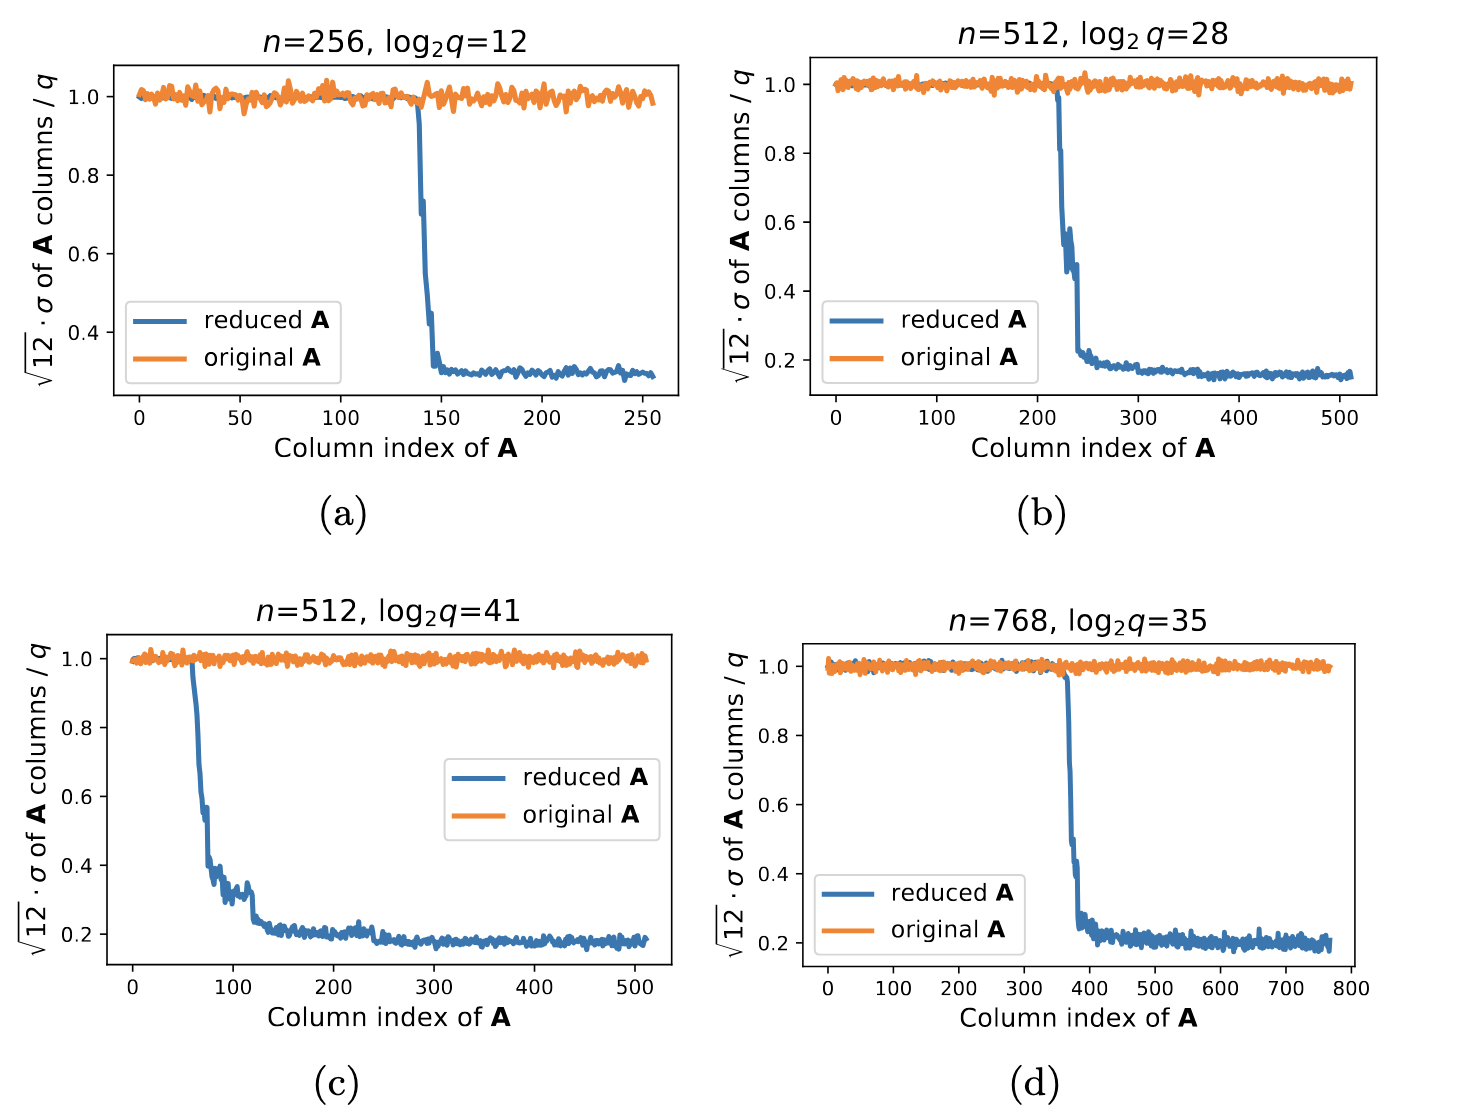
\includegraphics[width=0.7\linewidth]{example_variance_plot.png}
    \end{center}
  
    \scriptsize{
    \textbf{Conceptual Plot:}  
    The original $\mathbf{A}$ (orange) has uniform column variance $\approx q/\sqrt{12}$,
    while the reduced $\mathbf{A}'$ (blue) shows a significant drop after column index $n_u$.
    }
  \end{frame}

  \subsection*{Bit distinction: More details}
  % ----------------------------------------------------------------------------
\begin{frame}{Cruel vs. Cool Bits}
  \textbf{Cruel bits}:
  \begin{itemize}
    \item The $n_u$ unreduced columns (remain $\sim$uniform in $\mathbb{Z}_q$).
    \item Hard portion of the secret.
  \end{itemize}

  \textbf{Cool bits}:
  \begin{itemize}
    \item The $n_r = n - n_u$ reduced columns (low variance).
    \item Easy portion of the secret (recoverable with simple stats).
  \end{itemize}

  \vspace{0.3cm}
  \textbf{Key Observation}: 
  After partial reduction, the dot product $\mathbf{a}\cdot \mathbf{s}$ is dominated by
  the cruel bits if you guess them incorrectly. The correct guess yields a recognizable residual pattern, making it statistically distinguishable.
\end{frame}

\begin{frame}{Cruel Bit Brute Force}
  \textbf{Hardest step:}
  \begin{itemize}
    \item We only guess $\mathbf{s}_{0:n_u}$, the cruel portion.
    \item Evaluate
      \[
        \mathbf{R}\mathbf{A} \cdot \mathbf{s}^* - \mathbf{R}\mathbf{b} \pmod{q}
      \]
      for each guess $\mathbf{s}^*$ in that subspace.
    \item The \emph{correct guess} exhibits narrower standard deviation or a distinct residual distribution (as shown in next figure).
  \end{itemize}

  \vspace{0.4cm}
  \textbf{Why feasible?}  
  $n_u$ is significantly smaller than $n$; or the attacker knows $h_u$ (the smaller Hamming weight among the cruel bits).
\end{frame} 
% =========================
% Slide: Greedy Recovery of Cool Bits
% =========================
\section{Distinction of Bits and Variance Related}
\subsection*{Algorithm for Cool Bit Recovery}
\begin{frame}{Greedy Recovery of ``Cool'' Bits}
  % SPEAKER NOTES:
  % - Summarize how once the cruel bits are brute-forced, 
  %   the remainder (cool bits) can be handled by a simple flipping approach
  % - Optionally mention that it fails if columns have moderate variance.
  
  \textbf{Context:} From original paper, once $n_u$ ``cruel'' bits are correctly guessed, the remaining $n_r = n - n_u$ bits have lower variance, enabling a simple \emph{bit-flip} approach.
  
  \begin{algorithm}[H]
  \caption{\small Greedy Recovery of Cool Bits}
  \label{alg:greedy-cool}
  \footnotesize
  \begin{algorithmic}[1]
  \Require $\mathbf{s}^*$ partially correct (cruel bits), the rest set to 0
  \For{$i$ in $\{n - n_r,\dots,n-1\}$}
    \State $s^*[i] \gets 0$
    \State $\sigma_0 \gets \sigma(\mathbf{A}\cdot \mathbf{s}^* - \mathbf{b}\mod q)$
    \State $s^*[i] \gets 1$
    \State $\sigma_1 \gets \sigma(\mathbf{A}\cdot \mathbf{s}^* - \mathbf{b}\mod q)$
    \If{$\sigma_0 \le \sigma_1$}
      \State $s^*[i] \gets 0$
    \Else
      \State $s^*[i] \gets 1$
    \EndIf
  \EndFor
  \end{algorithmic}
  \end{algorithm}
  
  \end{frame}
  
  \subsection*{Std Deviation Showcase}
  \begin{frame}{Statistical Representation}
  \textbf{Residual Histogram Example:}
  \begin{center}
    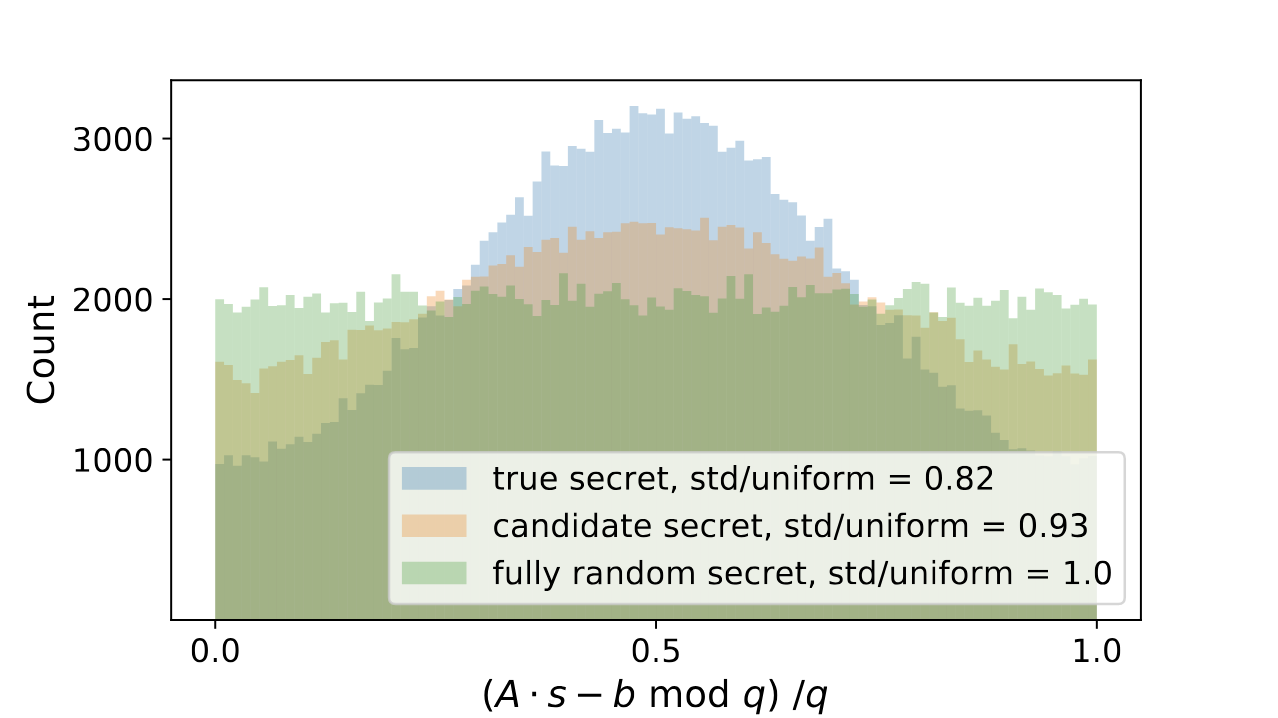
\includegraphics[width=0.8\textwidth]{residual_histogram.png}
  \end{center}
  {\scriptsize \textbf{Blue:} True secret guess, \textbf{Orange:} Partially correct guess, \textbf{Green:} Random guess.}
  \end{frame}
  
  % =========================
  % Slide: Variance Diagram & 3-Zone Rationale
  % =========================
  \begin{frame}{Variance Diagram Discussion}
  % SPEAKER NOTES:
  % - Show that partial-lattice reduction can yield a slope in the variance
  % - Introduce Cruel/Chill/Cool partition as a refined approach
  
  \textbf{Empirical Observation:}
  \begin{itemize}
    \item After partial lattice reduction, columns sometimes exhibit a \emph{gradual} drop in variance.
    \item A purely two-zone (Cruel vs.\ Cool) classification may fail if many columns have \emph{moderate} variance.
  \end{itemize}
  
  \begin{figure}[ht]
    \centering
    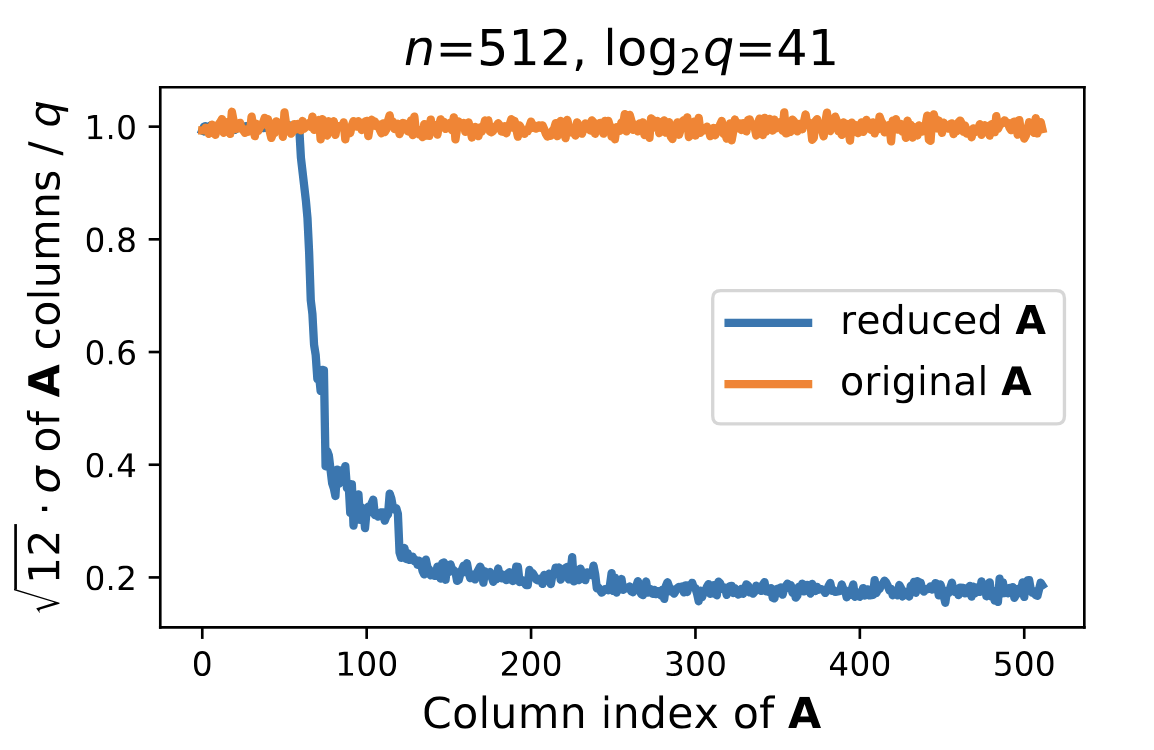
\includegraphics[width=0.45\linewidth]{512-41.png}
    \hfill
    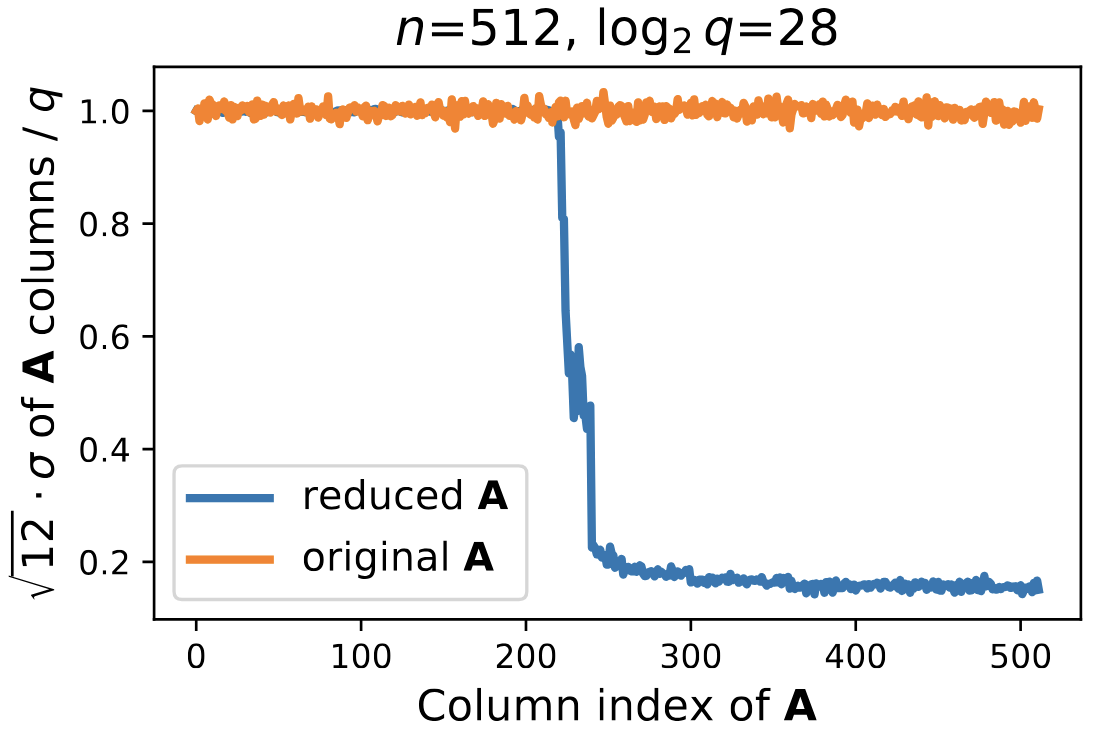
\includegraphics[width=0.45\linewidth]{512-28.png}
  \end{figure}
  \end{frame}
  

% --------------------------------------------------------------------------
\begin{frame}{Annotated Figures: Cruel, Chill, and Cool Regions}
  \begin{figure}[ht]
      \centering
      % Subfigure 1
      \begin{subfigure}{0.49\textwidth}
          \centering
          \begin{tikzpicture}
              \node[anchor=south west, inner sep=0] (image) at (0,0)
                {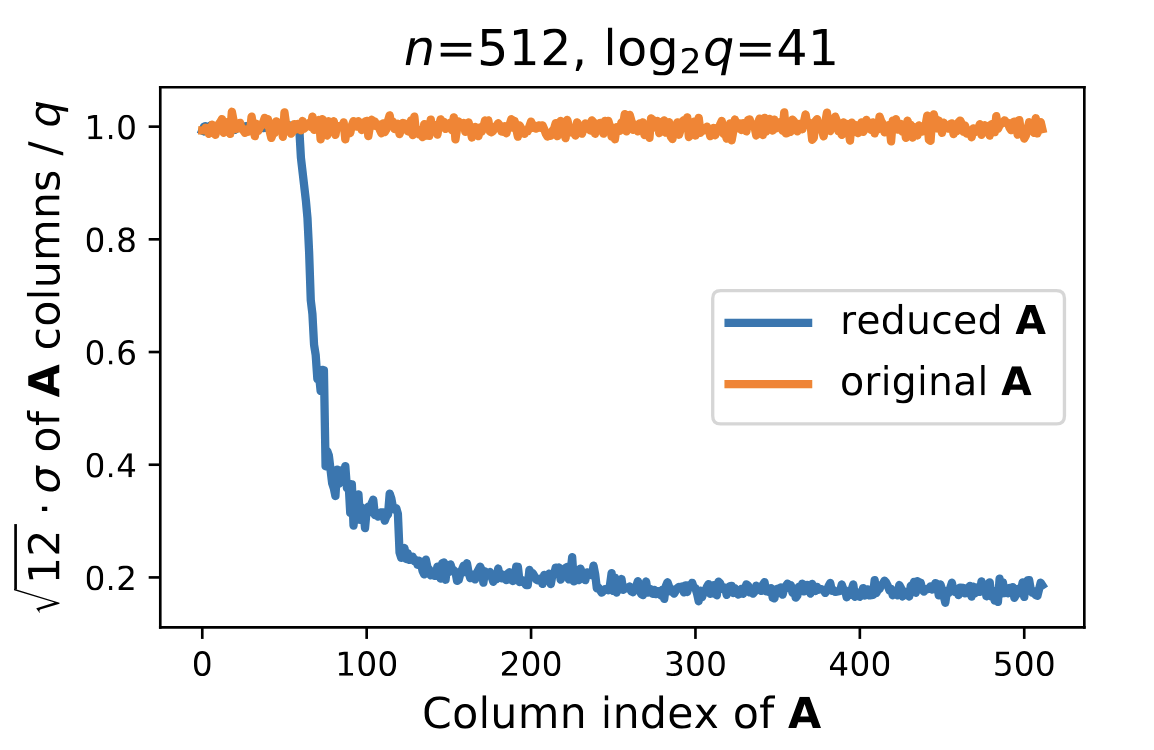
\includegraphics[width=\textwidth]{512-41.png}};
              \begin{scope}[x={(image.south east)}, y={(image.north west)}]
                  % Cruel region (green frame)
                  \draw[thick, green, fill=green!20, opacity=0.3] (0.18, 0.19) rectangle (0.28, 0.8);
                  % Chill region (yellow frame)
                  \draw[thick, yellow, fill=yellow!20, opacity=0.3] (0.285, 0.19) rectangle (0.345, 0.8);
                  % Cool region (blue frame)
                  \draw[thick, blue, fill=blue!20, opacity=0.3] (0.35, 0.19) rectangle (0.91, 0.8);
              \end{scope}
          \end{tikzpicture}
          \caption{\small $n=512,\,\log_2 q=41$.}
          \label{fig:region1}
      \end{subfigure}
      \hfill
      % Subfigure 2
      \begin{subfigure}{0.49\textwidth}
          \centering
          \begin{tikzpicture}
              \node[anchor=south west, inner sep=0] (image) at (0,0)
                {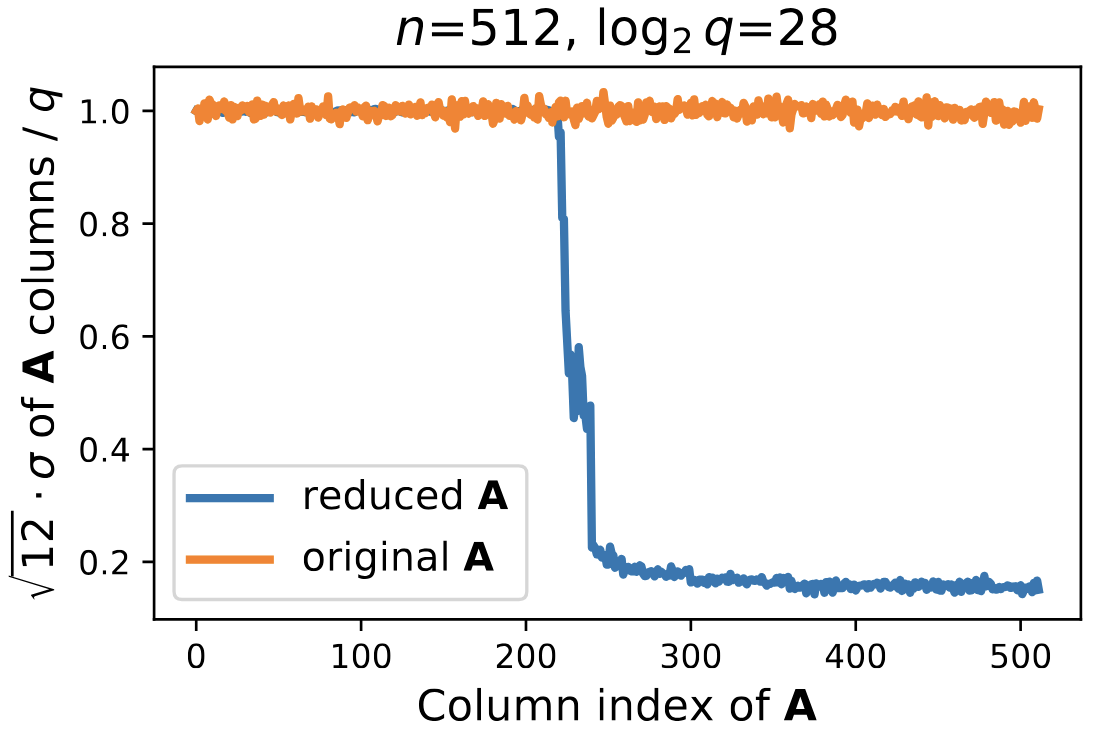
\includegraphics[width=\textwidth]{512-28.png}};
              \begin{scope}[x={(image.south east)}, y={(image.north west)}]
                  % Cruel region (green frame)
                  \draw[thick, green, fill=green!20, opacity=0.3] (0.18, 0.19) rectangle (0.505, 0.8);
                  % Chill region (yellow frame)
                  \draw[thick, yellow, fill=yellow!20, opacity=0.3] (0.510, 0.19) rectangle (0.525, 0.8);
                  % Cool region (blue frame)
                  \draw[thick, blue, fill=blue!20, opacity=0.3] (0.530, 0.19) rectangle (0.935, 0.8);
              \end{scope}
          \end{tikzpicture}
          \caption{\small $n=512,\,\log_2 q=28$.}
          \label{fig:region2}
      \end{subfigure}
      \caption{\small Division of columns into \textbf{Cruel} (green), \textbf{Chill} (yellow), and \textbf{Cool} (blue) zones,
      reflecting standard deviation changes post-reduction.}
      \label{fig:annotated_regions}
  \end{figure}
  \end{frame}
% --------------------------------------------------------------------------
\begin{frame}{Proposed Method: Threshold-Based Zoning}
  \textbf{Threshold Model:}
  
  Let $\sigma_j$ be the standard deviation of column $j$ in the reduced matrix $\mathbf{A}'$.
  Define two thresholds $T_c$ and $T_h$ such that
  \[
    T_c > T_h > 0, \quad \text{(e.g., }T_c \approx 0.8\,\sigma_u,\; T_h \approx 0.3\,\sigma_u\text{).}
  \]
  We classify each column $j$ by:
  \[
    \text{Region}(j) =
    \begin{cases}
      \mathrm{Cruel} & \text{if } \sigma_j \ge T_c, \\
      \mathrm{Chill} & \text{if } T_h \;\le\;\sigma_j < T_c, \\
      \mathrm{Cool}  & \text{if } \sigma_j < T_h.
    \end{cases}
  \]
  
  \textbf{Why This Works:}
  \begin{itemize}
    \item \(\sigma_j \approx q/\sqrt{12}\) $\rightarrow$ treat as Cruel, requiring heavy enumeration.
    \item \(\sigma_j \ll q/\sqrt{12}\) $\rightarrow$ treat as Cool, a small variance for easy per-bit flips.
    \item \(\sigma_j\) in-between $\rightarrow$ use a \emph{more refined} partial approach.
  \end{itemize}
  \end{frame}

  % =======================================
\section{Variance Diagram and 3-Zone Partition}
% =======================================

\subsection*{Why Does a Slope Appear?}
\begin{frame}{Why a Slope Might Appear}
% SPEAKER NOTES:
% - We point out partial-lattice reduction doesn't always produce a perfect "cliff."
% - Some columns get "semi-reduced" depending on how BKZ or flatter is interleaved.
% - Introduce idea of a "sloping region."

\textbf{Partial Lattice Reduction in Practice:}
\begin{itemize}
  \item Techniques like \texttt{flatter} and BKZ may alternate or stall, 
        producing columns that are \emph{partially} reduced.
  \item This leads to some columns having \textbf{medium} variance, 
        rather than a strict jump from $\approx q/\sqrt{12}$ to a low value.
\end{itemize}

\textbf{Observation:}
\begin{itemize}
  \item Instead of a neat ``cliff,'' we see a \emph{sloping} region
        in many empirical plots.
  \item Such semi-reduced columns are \emph{neither} trivially brute forced
        \emph{nor} trivially recovered by a single flip.
\end{itemize}

\bigskip
\textbf{Implication:} 
We need a more nuanced approach to handle these \emph{intermediate} columns effectively.
\end{frame}

% ============================================
\subsection*{Why a Three-Zone Partition?}
\begin{frame}{Arguing for Three Zones: Cruel, Chill, \& Cool}
% SPEAKER NOTES:
% - Show that a 2-zone "cool & cruel" approach fails if there's a big medium-variance portion.
% - Outline how we define a 3-zone partition, with Chill being the transitional region.

\vspace{0.2cm}
\textbf{Our Three-Zone Decomposition:}
\[
  \mathcal{I}_{\mathrm{cruel}},\ 
  \mathcal{I}_{\mathrm{chill}},\ 
  \mathcal{I}_{\mathrm{cool}}
  \;\subseteq\;\{1,\dots,n\}, 
  \quad
  \bigcup \text{ = all columns.}
\]
\begin{itemize}
  \item \textbf{Cruel (Green):} 
    High-variance columns needing brute force or partial guesses.
  \item \textbf{Chill (Yellow):} 
    Transitional \emph{sloping} columns, tackled with \emph{probabilistic or ML-based} enumerations.
  \item \textbf{Cool (Blue):} 
    Fully reduced columns, recovered by a simple \textbf{greedy flip}.
\end{itemize}

\vspace{0.2cm}
\textbf{Motivation:}
\begin{itemize}
  \item \emph{Reduced Overhead:} Limit brute force to truly uniform columns.
  \item \emph{Structured Data:} Medium-variance columns can still be partially distinguished by advanced methods.
  \item \emph{Adaptive Windowing:} Possibly shrink or expand Chill as needed.
\end{itemize}
\end{frame}

\section{Matrix Partition Examples}

\subsection*{Unmultiplied Example}
\begin{frame}{Example Matrix Partition (I)}
% SPEAKER NOTES:
% - Show how columns are color-coded as Cruel, Chill, and Cool.
% - This first image does NOT multiply by s or add error e.

\begin{figure}[ht]
  \centering
  % Replace 'width=0.7\linewidth' if you prefer a different size
  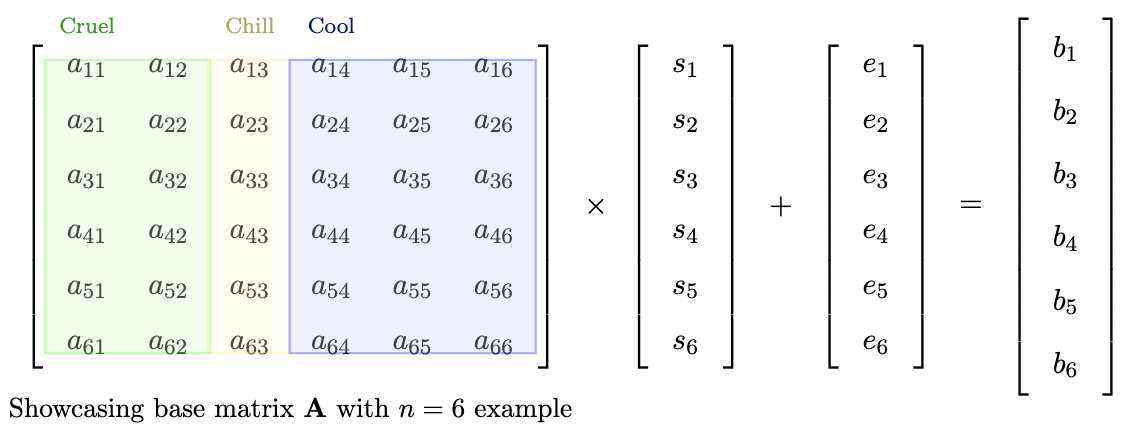
\includegraphics[width=0.7\linewidth]{unmultiplied.png}
  \caption{\small Conceptual $n \times n$ matrix with columns labeled \textbf{Cruel} (green), 
  \textbf{Chill} (yellow), and \textbf{Cool} (blue).}
  \label{fig:unmultiplied_partition}
\end{figure}

\textbf{Note:} 
\begin{itemize}
  \item We highlight columns in green/yellow/blue to illustrate partial-lattice reduction outcome.
  \item High-variance columns (Cruel) vs.\ transitional (Chill) vs.\ reduced (Cool).
\end{itemize}

\end{frame}


\subsection*{Multiplied Example}
\begin{frame}{Example Matrix Partition (II)}
% SPEAKER NOTES:
% - This second image includes multiplication by s and addition of e, showing b = A*s + e.

\begin{figure}[ht]
  \centering
  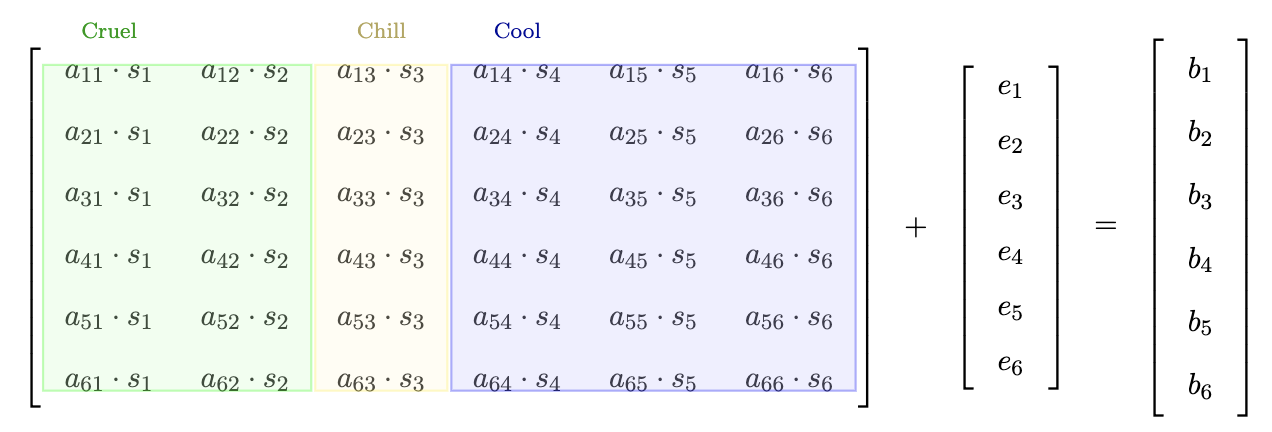
\includegraphics[width=0.7\linewidth]{multiplied.png}
  \caption{\small Element-wise multiplication of $\mathbf{A}$ by $\mathbf{s}$ plus error $\mathbf{e}$,
    illustrating \textbf{Cruel}, \textbf{Chill}, and \textbf{Cool} columns.}
  \label{fig:multiplied_partition}
\end{figure}

\textbf{Note:}
\begin{itemize}
  \item Each column remains colored based on variance classification.
  \item The final vector $\mathbf{b}$ is formed as $\mathbf{b} = \mathbf{A}\mathbf{s} + \mathbf{e}$.
\end{itemize}

\end{frame}

% -------------------------------------------
\section{Attack Showcase}
% -------------------------------------------

\subsection*{Attack Phases}
\begin{frame}{Three Attack Phases}
% SPEAKER NOTES:
% - Outline each phase: Cruel brute force, Chill probabilistic enumeration, 
%   Cool greedy approach. Keep short.

\textbf{Phase 1: Brute Force (Cruel)}
\begin{itemize}
  \item Columns in $\mathcal{I}_{\mathrm{cruel}}$ have variance $\approx \frac{q}{\sqrt{12}}$.
  \item Must guess bits, e.g., $\mathrm{BruteForceCruel}(\mathbf{A}_{*, \mathcal{I}_{\mathrm{cruel}}}, \mathbf{b})$.
  \item Let $\mathbf{s}_{\mathrm{cruel}}$ be recovered cruel bits; 
        $\mathrm{cruel\_ones} = \mathrm{HW}(\mathbf{s}_{\mathrm{cruel}})$.
\end{itemize}

\textbf{Phase 2: Probabilistic (Chill)}
\begin{itemize}
  \item \emph{Chill} region $\mathcal{I}_{\mathrm{chill}}$ has moderate variance.
  \item Assign $p_j = \mathrm{EstimateProb}(j,\mathbf{A},\mathbf{s}_{\mathrm{cruel}})$. 
  \item Select $k = h - \mathrm{cruel\_ones}$ bits to be 1.
  \item Possibly refine guess with local flips if final check fails.
\end{itemize}

\textbf{Phase 3: Greedy (Cool)}
\begin{itemize}
  \item $\mathcal{I}_{\mathrm{cool}}$ columns: significantly reduced variance.
  \item Use \textbf{GreedyFlip} approach: flip bit if it lowers residual variance.
\end{itemize}
\end{frame}


\subsection*{Pseudocode}
\begin{frame}{Multi-Zone Attack Algorithm}
% SPEAKER NOTES:
% - Display the code snippet for the 3-zone approach. 
%   Provide minimal bullet commentary.

\textbf{Algorithm: Cool, Chill, \& Cruel}
\small
\begin{algorithm}[H]
\caption{\small Multi-Zone Recovery}
\label{alg:ccc-attack}
\begin{algorithmic}[1]
\Require Reduced $\mathbf{A}$, vector $\mathbf{b}$, $q$, Hamming weight $h$
\State $(\mathcal{I}_{\mathrm{cruel}},\mathcal{I}_{\mathrm{chill}},\mathcal{I}_{\mathrm{cool}}) \gets \text{ClassifyColumns}(\mathbf{A}, T_c, T_h)$
\State $\mathbf{s}_{\mathrm{cruel}} \gets \mathrm{BruteForceCruel}(\mathbf{A}_{*,\mathcal{I}_{\mathrm{cruel}}}, \mathbf{b})$
\State $\mathrm{cruel\_ones} \gets \mathrm{HW}(\mathbf{s}_{\mathrm{cruel}})$
\State $p_j \gets \mathrm{EstimateProb}(j,\mathbf{A},\mathbf{s}_{\mathrm{cruel}}),\ j\in \mathcal{I}_{\mathrm{chill}}$
\State $k \gets h - \mathrm{cruel\_ones}$
\State $\mathbf{s}_{\mathrm{chill}} \gets \mathrm{RankAndAssign}(p_j,\ k)$
\State $\mathbf{s}_{\mathrm{cool}} \gets \mathrm{GreedyFlip}(\mathbf{A},\mathbf{b},\mathbf{s}_{\mathrm{cruel}},\mathbf{s}_{\mathrm{chill}})$
\State $\mathrm{RefineChill}(\mathbf{A},\mathbf{b},\mathbf{s}_{\mathrm{cruel}},\mathbf{s}_{\mathrm{chill}},\mathbf{s}_{\mathrm{cool}})$
\State \textbf{return} $(\mathbf{s}_{\mathrm{cruel}}, \mathbf{s}_{\mathrm{chill}}, \mathbf{s}_{\mathrm{cool}})$
\end{algorithmic}
\end{algorithm}

\end{frame}

\subsection*{Notes to attack algorithm}

\begin{frame}
\textbf{Key Points:}
\begin{itemize}
  \item \textproc{EstimateProb} uses variance or small ML models to rank bits in \emph{Chill}.
  \item \textproc{GreedyFlip} is the standard bit-flip from earlier slides.
  \item \textproc{RefineChill} tries local flips if the guess fails final checks.
\end{itemize}
\end{frame}

% =======================================
\section{Mathematical and Logical Details}
\label{sec:math-logic}
% =======================================

\subsection*{Probability \& Combinatorial Logic (Slide 1)}
\begin{frame}{Probability \& Combinatorial Logic}
% SPEAKER NOTES:
% - Introduce how we pick the Chill bits, how many remain after Cruel is enumerated.
% - Outline the concept of p_j for each column.

\textbf{Partition Counts:}
\begin{itemize}
  \item After partial-lattice reduction, columns split into $\mathcal{I}_{\mathrm{cruel}}, \mathcal{I}_{\mathrm{chill}}, \mathcal{I}_{\mathrm{cool}}$.
  \item Let $n_{\mathrm{cruel}}, n_{\mathrm{chill}}, n_{\mathrm{cool}}$ be the respective counts.
  \item Once the $\mathrm{cruel}$ bits are guessed, define 
    \[
      \mathrm{cruel\_1} = \mathrm{HW}(\mathbf{s}_{\mathrm{cruel}}), 
      \quad
      k = h - \mathrm{cruel\_1}.
    \]
    Here, $k$ bits remain for Chill + Cool.
\end{itemize}

\textbf{Probability-Based Ranking (Chill):}
\begin{itemize}
  \item For each column $j \in \mathcal{I}_{\mathrm{chill}}$, assign $p_j = \Pr[s_j = 1]$.
  \item E.g., a heuristic $p_j \propto 1/\sigma_j$, or a small ML model, or a direct statistical test.
  \item Select $k_{\mathrm{chill}} \le k$ columns with highest $p_j$ as 1; place the rest in $\mathcal{I}_{\mathrm{cool}}$.
\end{itemize}

\end{frame}


\subsection*{Local Search \& Refinement (Slide 2)}
\begin{frame}{Local Search \& Refinement}
% SPEAKER NOTES:
% - If the final guess fails, we do partial BFS or flips to correct borderline bits in Chill.

\textbf{Local Search If Guess Is Wrong:}
\begin{itemize}
  \item Even with probability ranking, some columns may be misclassified.
  \item A small BFS or iterative flip approach can fix borderline columns without enumerating all 
    $\binom{n_{\mathrm{chill}}}{k_{\mathrm{chill}}}$ subsets.
\end{itemize}

\textbf{Example Strategy:}
\begin{itemize}
  \item \textbf{RefineChill}:
    \begin{enumerate}
      \item Identify columns $j$ with $p_j$ near threshold.
      \item Try flipping a bit from 0 to 1 (or 1 to 0).
      \item Re-check residual distribution or variance $\sigma(\mathbf{A}\mathbf{s}^* - \mathbf{b})$.
      \item Keep flip if it improves correctness, discard otherwise.
    \end{enumerate}
  \item Repeat until no improvement or iteration limit reached.
\end{itemize}

\textbf{Goal:}
\begin{itemize}
  \item Achieve high success rate on Chill bits without \emph{full} enumeration.
  \item Balance overhead vs.\ accuracy in partial-lattice cryptanalysis.
\end{itemize}
\end{frame}

% -------------------------------------------
\subsection*{Complexity Insights}
\begin{frame}{Complexity: Overview and Formula}
% SPEAKER NOTES:
% - Introduce the approximate cost:
%   (1) brute force for Cruel,
%   (2) enumerations in Chill,
%   (3) minimal overhead for Cool.

\textbf{Overall Cost:}
\begin{itemize}
  \item \emph{Cruel} brute force, e.g.\ $2^{n_{\mathrm{cruel}}}$,
  \item \emph{Chill} enumerations or partial BFS,
  \item \emph{Cool} overhead, typically linear in $n_{\mathrm{cool}}$.
\end{itemize}

\bigskip
\textbf{Notional Complexity Formula:}
\begin{center}
  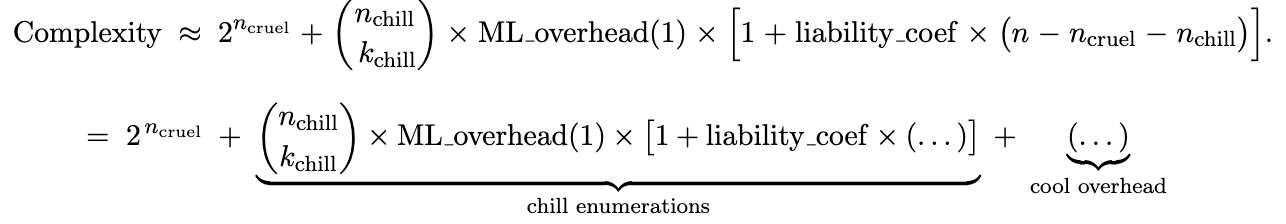
\includegraphics[width=1\linewidth]{Complexity.png}
\end{center}
{\scriptsize (Schematic of the main terms: $2^{n_{\mathrm{cruel}}}$, $\binom{n_{\mathrm{chill}}}{k_{\mathrm{chill}}}$, $\mathrm{ML\_overhead}(1)$, etc.)}

\end{frame}

\begin{frame}{Complexity: Explanation}
\textbf{Term-by-Term Explanation:}
\begin{enumerate}
  \item $2^{n_{\mathrm{cruel}}}$: Exhaustive or MITM for high-variance columns.
  \item $\binom{n_{\mathrm{chill}}}{k_{\mathrm{chill}}}$: 
        Worst-case enumerations in Chill (often reduced by ranking/BFS).
  \item $\mathrm{ML\_overhead}(1)$: 
        Extra cost per candidate if using neural nets or advanced tests.
  \item $\mathrm{liability\_coef}\times(\dots)$: 
        Local flips or expansions upon guess failure.
  \item \textbf{Cool overhead}: $O(n_{\mathrm{cool}})$ from final bit-flip.
\end{enumerate}
\end{frame}


% -------------------------------------------
% Slide: Complexity Insights (II)
% -------------------------------------------
\subsection*{Complexity Insights}
\begin{frame}{Comparison to Original Cool \& Cruel Approach}
% SPEAKER NOTES:
% - Contrast with the 2-zone model from "Cool & Cruel" which has complexity ~ 2^n_u + O(n - n_u).
% - Highlight that your method invests partial enumerations for the Chill region, possibly lowering n_cruel.

\textbf{Original Two-Zone Complexity}:
\[
  2^{\,n_u} 
  \;+\; O\bigl(n - n_u\bigr),
  \quad
  n_u \approx n_{\mathrm{cruel}}.
\]
\begin{itemize}
  \item Columns are \emph{either} fully brute forced or trivially flipped.
  \item Medium-variance columns can inflate $n_u$ or cause repeated flips.
\end{itemize}

\vspace{0.3em}
\textbf{Our Three-Zone Method:}
\begin{itemize}
  \item Potentially lowers $n_{\mathrm{cruel}}$ by pushing some columns into the \emph{Chill} set,
  \item Incur extra $\binom{n_{\mathrm{chill}}}{k_{\mathrm{chill}}}$ overhead 
        but less brute force dimension overall.
  \item If the slope region is large, partial enumerations or ML can be more efficient than a huge $2^{\,n_u}$.
\end{itemize}

\textbf{Conclusion:}
\begin{itemize}
  \item \emph{If} columns form a clear cliff, two-zone is simpler.
  \item \emph{If} a slope is substantial, three-zone yields better scaling in practice.
\end{itemize}
\end{frame}



% =============================================
\section{Discussion, Future Work, and Conclusion}
% =============================================

\subsection*{Discussion (Slide 1)}
\begin{frame}{Discussion: Three-Zone Approach}
% SPEAKER NOTES:
% - Summarize how the 3-zone approach addresses slope issues in partial-lattice reduction.

\textbf{Three-Zone Motivation:}
\begin{itemize}
  \item Columns after reduction may not show a perfect ``cliff'' in variance.
  \item We introduce a \textbf{Chill} region for moderate-variance columns, 
        bridging pure brute force (Cruel) and trivial bit-flip (Cool).
\end{itemize}

\textbf{Method Highlights:}
\begin{itemize}
  \item \emph{Cruel subset:} brute force or meet-in-the-middle.
  \item \emph{Chill subset:} probabilistic or ML-driven ranking.
  \item \emph{Cool subset:} final greedy bit-flip step.
\end{itemize}

\textbf{Complexity Recap:}
\begin{itemize}
  \item Chill enumerations can reduce an otherwise large brute force dimension.
  \item Overhead arises from classification or local refinement (Section~\ref{sec:math-logic}).
\end{itemize}
\end{frame}


\subsection*{Discussion (Slide 2)}
\begin{frame}{Balancing Lattice Reduction}
% SPEAKER NOTES:
% - Mention stronger partial reduction reduces n_cruel but increases noise,
%   referencing the existing idea from the original cool-and-cruel paper.

\textbf{Key Observation}:
\begin{itemize}
  \item Stronger reduction $\implies$ fewer cruel bits ($n_{\mathrm{cruel}}$), 
        but larger noise $\sigma_e$ for Chill/Cool.
  \item We can tune penalty param $\omega$ and block sizes in BKZ/\texttt{flatter}
        to find an optimal middle ground.
\end{itemize}

\textbf{Future Experiments Needed:}
\begin{itemize}
  \item Measure trade-off between enumerating more cruel bits vs.\ coping 
        with bigger noise in Chill/Cool.
  \item Possibly adapt or incrementally choose $\omega$ mid-process
        if the slope region is large.
\end{itemize}
\end{frame}


\subsection*{Future Work (Slide 3)}
\begin{frame}{Future Work}
% SPEAKER NOTES:
% - Present the main bullet points on Ternary/Gaussian secrets, synergy with SALSA, etc.

\textbf{1. Ternary/Gaussian Secrets}
\begin{itemize}
  \item Many HE systems use ternary or narrow Gaussian distributions.
  \item Chill-based classification needs adjusted probability models or ML training.
\end{itemize}

\textbf{2. Combining with SALSA/Transformers}
\begin{itemize}
  \item SALSA, PICANTE, VERDE show ML can recover bits efficiently.
  \item Our Chill region could adopt such models, but overhead must remain manageable.
\end{itemize}

\textbf{3. Real-World Library Impact}
\begin{itemize}
  \item HE libs (HElib, SEAL) use small/sparse secrets.
  \item Mitigations include randomizing secret distribution or sub-lattice rotations.
\end{itemize}

\textbf{4. Parameter Tuning \& Local Search}
\begin{itemize}
  \item Defining “liability coefficients,” iteration limits for flips in Chill remains open.
  \item Tuning approach to get practical speedups is crucial.
\end{itemize}

\textbf{5. Expanding the Chill Window}
\begin{itemize}
  \item Iteratively adjust which columns fall into Chill vs.\ Cool.
  \item Evaluate performance on borderline columns.
\end{itemize}
\end{frame}


\subsection*{Conclusion (Slide 4)}
\begin{frame}{Conclusion}
% SPEAKER NOTES:
% - Summarize the new approach and highlight next steps.

\textbf{Cool, Chill, and Cruel Partition}:
\begin{itemize}
  \item Addresses limitations of a purely two-zone partial-lattice attack.
  \item Each subset (Cruel, Chill, Cool) uses a method suited to its variance regime.
\end{itemize}

\textbf{Key Takeaways}:
\begin{itemize}
  \item The Chill region adds overhead but can dramatically reduce brute force size.
  \item Fine-tuning partial reduction ($\omega$) and local search heuristics is essential.
  \item Empirical tests up to $n=1024$ will confirm practicality for real HE systems.
\end{itemize}

\textbf{Looking Ahead:}
\begin{itemize}
  \item Further synergy with ring-based LWE and advanced ML classification.
  \item Bridging classical cryptanalysis and modern ML to break small/sparse LWE secrets.
\end{itemize}

\end{frame}



% ----------------------------------------------------------------------------
\begin{frame}{References}
  \footnotesize
  \begin{thebibliography}{9}
    \bibitem{regev}
    O. Regev. \emph{On Lattices, Learning with Errors, Random Linear Codes, and Cryptography.} J. ACM 51(6), 2005.

    \bibitem{concrete_results}
    Niklas N., ...
    \emph{The Cool and the Cruel: Separating Hard Parts of LWE Secrets., https://eprint.iacr.org/2024/443.pdf}
    (ArXiv, 2024).
    
    \bibitem{someRef2}
    Albrecht et al. \emph{Estimate all the LWE, NTRU schemes.  https://eprint.iacr.org/2018/331} (2018).

    \bibitem{BKZ2ref}
    Chen, Y., Nguyen, P. Q.,
    \emph{BKZ 2.0: Better Lattice Security Estimates}.
    Lecture Notes in Computer Science, 2011.

    \bibitem{FlatterRef}
    Ryan, K., Heninger, N.
    \emph{Fast practical lattice reduction through iterated compression.}
    Annual International Cryptology Conference. Springer, 2023.

    \bibitem{PolishRef}
    Charton, F., Lauter, K., Li, C., Tygert, M.
    \emph{An efficient algorithm for integer lattice reduction. SIAM Journal on Matrix Analysis and Applications}
    (2024).

    \bibitem{SALSAref}
    Gama, N., Ducas, L. et al.,
    \emph{On SALSA Picante ML Attack Method. https://eprint.iacr.org/2023/340} (2023).
    % Add more references as needed
  \end{thebibliography}
\end{frame}

% ----------------------------------------------------------------------------
\end{document}
